\chapter{Validation}
\label{chapter:evaluation}
In this chapter we present the accuracy and the scalability experiments we performed to evaluate the implemented flow-level model. As we outlined in our method chapter, we compare our implementation with the packet-level implementation of ECOFEN (based on NS-3).  
\section{Experiment Setup}
For all our experiments the version of NS-3 we used is version 3.26 and that of SimGrid is version 3.15. 
\subsection{General ECOFEN related setup}
Among the three power consumption models available in ECOFEN module, we used the \emph{linear} one. This model accepts idle power consumption values in Watts and also energy consumption values for each Byte received or send in nanoJoule. Throughout our experiments we used 10.3581 Watt as idle power consumption value and 3.423 nJ as Byte energy consumption value. We took these values from \cite{Sivaraman}, even though any arbitrary values can also suffice for our purpose.

The linear model estimates power consumption value for a given NIC (or NetDevice in NS-3's term) based on these two inputs and the amount of transmitted or received traffic. It then displays the estimated power consumption in Watt at specified time interval. We set the interval to be 0.05 sec (20 estimations per second) in order to get more frequent power estimation. 

What we want to get from ECOFEN is the total amount of energy consumed by the simulated network. To get this value, we first compute the average power drawn by the network for a given data transfer task and when the task ends, we multiply the average total network power with the data transfer time. 

\subsection{General SimGrid related setup}
For all of our experiments, we used a simple client/server SimGrid application. As described in Chapter~\ref{chapter:environment}, a typical SimGrid script contains three sections. Accordingly in our script, the first section represents what the client function does to send data. It simply accepts the number of Bytes to send from command line option or uses a default 1,000 Bytes if no value is specified, or it will generate the Bytes if random option is specified in the command line. Then it passes the Bytes to the SimGrid's send routine. By default there will be only one TCP flow for the specified Bytes, but if we want to send multiple flows we can also specify the number of flows on the command line. The server function simply issues the receive routine if there is data to receive. The third section, in addition to doing the tasks specified in Chapter~\ref{chapter:environment},  it is also a gateway to NS-3 or our implemented flow-level model depending on the option specified in the command line. 

For the link tag in SimGrid's platform file we used 10 Mbps  as a bandwidth value. This value is chosen because it falls within the range where ECOFEN's and SimGrid's simulated time value match closely as we have described by the end of Chapter~\ref{chapter:implementation}. For latency we used 10 ms and as a Watt-range power consumption value, we used 10.3581 Watt as idle power consumption value and 10.7479 Watt as a busy power consumption value. 

SimGrid's interface to NS-3 will set these bandwidth and latency values, together with other parameters, to NS-3's configuration. It means that we have only one SimGrid script to run both simulations (flow-based in SimGrid directly and packet-level in NS-3 with ECOFEN), thus ensuring a fair comparison on the same simulated network with the same generated traffic. 

\section{Accuracy Validation}
Our first objective consists in evaluating the accuracy of SimGrid's energy consumption estimates (done with our energy flow-based model) against the values computed by ECOFEN.
For this accuracy validation, we conduct two sets of experiments. In the first set, our purpose is to investigate the accuracy of energy consumption estimation difference between ECOFEN and the flow-level model when the size of platform changes. In SimGrid case, it means when the number of links change; in ECOFEN case, when the number of Nodes, NetDevices and the connection between them change. For this experiment we keep the number of flows and the data volume fixed but we increase the number of Links. In the second set, on the other hand, our purpose is to study the difference between the estimated energy consumption value between ECOFEN and SimGrid when the data size or flow changes while keeping the number of links fixed. Table~\ref{table:accuracyscenarios} shows all the tested scenarios and Figure~\ref{fig:sgvsns3scenario} shows the energy consumption prediction behavior of the implemented model and ECOFEN's model for all of the scenarios summarized in Table~\ref{table:accuracyscenarios}.

\begin{table}
	\begin{tabular}{|>{\centering\arraybackslash}m{1.6cm}|>{\centering\arraybackslash}m{1.8cm}|>{\centering\arraybackslash}m{1.9cm}|>{\centering\arraybackslash}m{1.8cm}|>{\centering\arraybackslash}m{2.2cm}|>{\centering\arraybackslash}m{1.6cm}|} 
		\hline 
	\textbf{Scenario} &	\textbf{Number of Links} & \textbf{Number of Flows} & \textbf{Data size(MB)} & \textbf{Bandwidth (Mbps)}& \textbf{Latency (ms)}\\ 
		\hline 
		1L1F&1&1&[20,500]&10&10\\
		\hline
		1L2F&1&2&[20,500]&10&10\\ 
		\hline
		1L4F&1&4&[10,100]&10&10\\ 
		\hline	 
		3L1F&3&1&[20,200]&10&10\\ 
		\hline
		3L2F&3&2&[20,100]&10&10\\ 
		\hline
	\end{tabular} 
	\caption{Scenarios tested for accuracy validation of the implemented flow-level model against ECOFEN. In the first column L stands for Link and F stands for Flow, hence 1L1F stands for one-link/one-flow scenario.}
	\label{table:accuracyscenarios}
\end{table}

In order to compare the energy consumption prediction accuracy of our flow-level model compared to the packet-level model of ECOFEN, we employed the unequal variance t-test method (a.k.a Welch's t-test) as suggested in~\cite{ruxton2006unequal}. The reason for choosing this test is that for our data sets obtained from the two simulators, we cannot assume equal variance, as the two data sets are independent. Table~\ref{table:welchtest} contains the statistics obtained from this test using R's built in Welch t-test function. 

\begin{figure}[htbp]
	\centering
	\subfigure[1 Link 1 Flow]{
		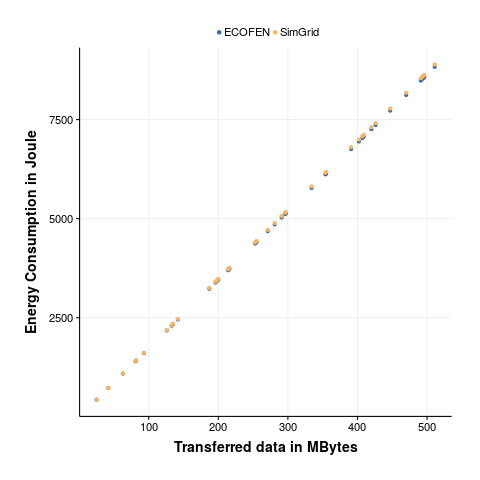
\includegraphics[width=0.45\linewidth]{images/ex11_energy_sg_vs_ns3}
		\label{fig:1l1f}
	}%
\centering
	\subfigure[1 Link 2 Flows]{
		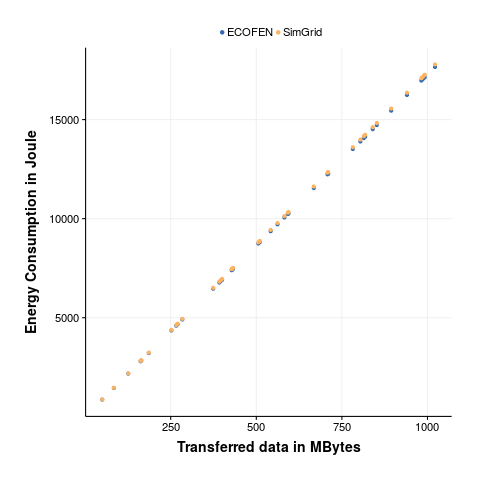
\includegraphics[width=0.45\linewidth]{images/ex12_energy_sg_vs_ns3}
		\label{fig:1l2f}
	}%
	
	\subfigure[1 Link 4 Flows]{
		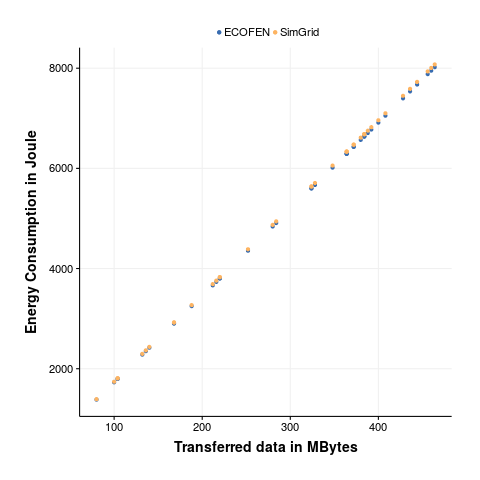
\includegraphics[width=0.45\linewidth]{images/ex10_energy_sg_vs_ns3}
		\label{fig:1l4f}
	}%
\centering
	\subfigure[3 Link 1 Flows]{
		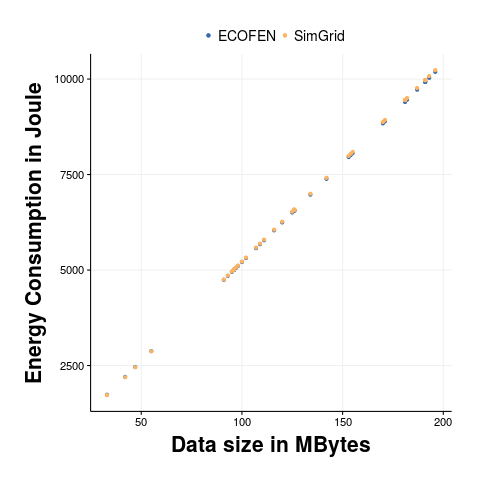
\includegraphics[width=0.45\linewidth]{images/ex13_energy_sg_vs_ns3}
		\label{fig:3l1f}
	}%

	\subfigure[3 Link 2 Flows]{
			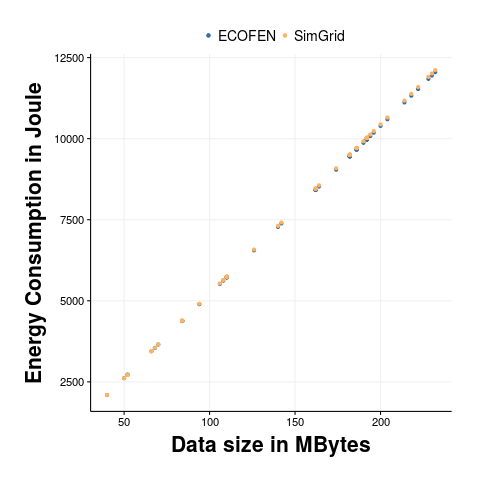
\includegraphics[width=0.45\linewidth]{images/ex15_energy_sg_vs_ns3}
			\label{fig:3l2f}
		}%
	\caption{Predicted energy consumption comparison of ECOFEN (blue dots) and SimGrid (orange dots) as a function of transferred Bytes for different path length and flow amount.}
	\label{fig:sgvsns3scenario}
\end{figure}
For all accuracy scenarios that we have tested, Figure~\ref{fig:sgvsns3scenario} demonstrates the closeness in energy consumption estimation between the implemented flow-level model and the packet-level model used for validation. From the last column of Table~\ref{table:welchtest} we can see that the maximum estimation error that our flow-level model registered is approximately 0.3\%, which is a very good estimation. The P-values shown in the fifth column also confirms that there is no statistically significant difference between the flow-level and the packet-level estimation.
\begin{table}
	\begin{tabular}{|>{\centering\arraybackslash}m{1.6cm}|>{\centering\arraybackslash}m{1.9cm}|>{\centering\arraybackslash}m{1.8cm}|>{\centering\arraybackslash}m{3.0cm}|>{\centering\arraybackslash}m{1.1cm}|>{\centering\arraybackslash}m{1.6cm}|} 
		\hline 
		\textbf{Scenario} &	\textbf{Mean of ECOFEN}&\textbf{Mean of SimGrid} & \textbf{CI  of Difference in mean} & \textbf{P-value}& \textbf{\% of Difference}\\ 
		\hline 
		1L1F&4837.2&4869.6&[-1156.3,1091.5]&0.9544&0.283\\
		\hline
		1L2F& 9672.6&9739.0& [-2314.2,2181.3]&0.9532&0.295\\ 
		\hline
		1L4F&5250.8&5286.9& [-720.10,647.90]&0.9169&0.297\\ 
		\hline	 
		3L1F&6804.9&6828.8& [-1024.9,977.1]&0.9622&0.124\\ 
		\hline
		3L2F&7896.6& 7931.9& [-1061.4,990.6]&0.9457&0.168\\ 
		\hline
	\end{tabular} 
	\caption{Unequal variance t-test statistics obtained using R. The confidence interval (CI) values in the fourth column are computed for the difference of the two energy consumption estimations and the last column values are obtained from mean log error as explained in \cite{DBLP:journals/tomacs/VelhoSCL13}.}
	\label{table:welchtest}
\end{table}

\section{Scalability Validation}
For validating the scalability of the implemented flow-level model, we run also two sets of experiments. In the first set, our goal is to investigate the scalability of the model when the path length increases. For these experiments we use path length values of 1, 2, 4, 6, 8 and 10. We fix the number of flows at 2 and the data size at 200 MB. In the second set, we examine the scalability as the data size increases. In this case, we keep the path length at 1 and the number of flows at 2, but we vary the data size randomly between 50 and 550 MB. The total number of data size values within this range was 21. 

Both of these experiments were carried out using the Grid'5000 testbed, supported by a scientific interest group hosted by Inria and including CNRS, RENATER and several Universities as well as other organizations\footnote{https://www.grid5000.fr/mediawiki/index.php/Grid5000:UsagePolicy}. The machine we used is SUN FIRE X2270 which have Intel Xeon X5570 2.93 GHz 2 CPUs, 4 cores per CPU and 24 GB RAM running Debian version 8 (jessie) operating system.

For each set of experiments, we use the Debian command, /usr/bin/time, to collect simulation run time and peak memory usage data. We run each experiment within each set seven times i.e., 7 run for each link in the first set and 7 run for each data size in the second set. Figure~\ref{fig:scallinks} shows the runtime and memory usage comparison as the path length increases. Figure~\ref{fig:scaldata}, on the other hand, shows the runtime and peak memory usage comparison as the data size increases.

\begin{figure}[ht]
	\centering
	\subfigure[Runtime]{
		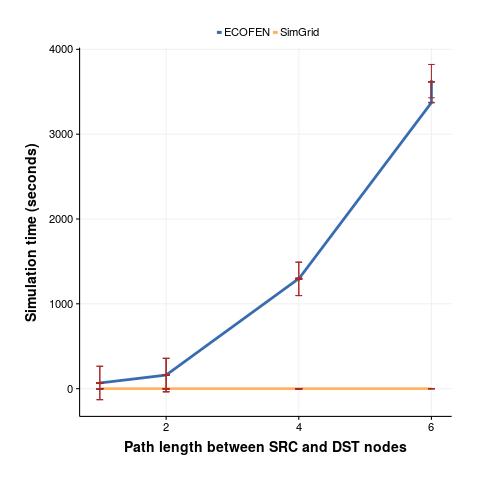
\includegraphics[width=0.5\linewidth]{images/ex16_linksize_sg_vs_ns3}
		\label{fig:lnkruntime}
	}%
	\centering
	\subfigure[Peak Memory Usage]{
		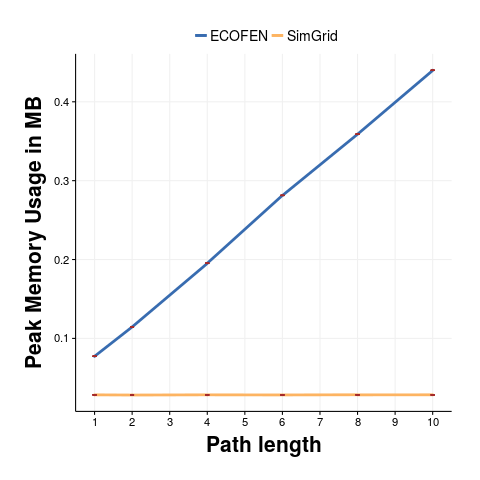
\includegraphics[width=0.5\linewidth]{images/ex16_linksizeM_sg_vs_ns3}
		\label{fig:lnkmem}
	}%
	\caption{Run time and peak memory usage comparison of ECOFEN and the flow-level model as the path length increases. In the figure the confidence interval for each experiment is also shown as a bar.}
	\label{fig:scallinks}
\end{figure}

\begin{figure}[ht]
	\centering
	\subfigure[Runtime]{
		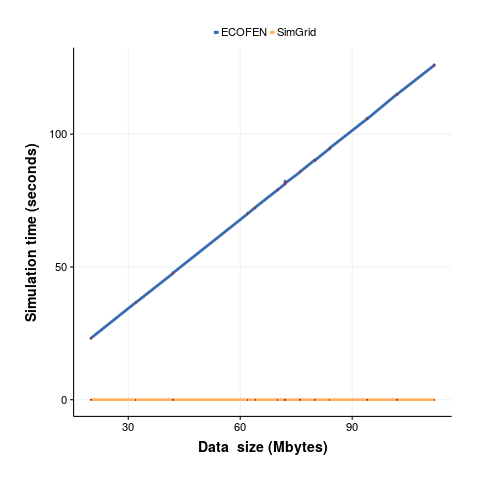
\includegraphics[width=0.47\linewidth]{images/ex21_datasize_sg_vs_ns3}
		\label{fig:datruntime}
	}%
	\centering
	\subfigure[Peak Memory Usage]{
		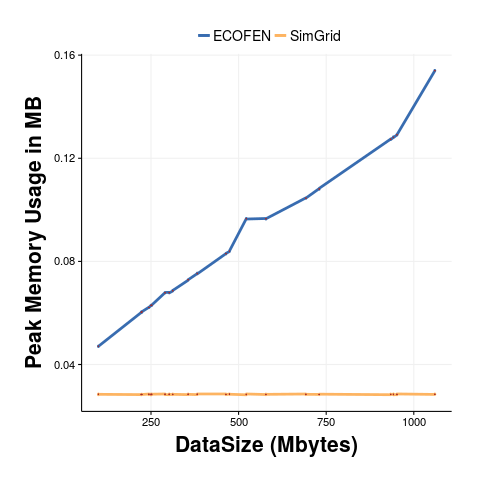
\includegraphics[width=0.47\linewidth]{images/ex21_DataSizeM_sg_vs_ns3}
		\label{fig:datmem}
	}%
	\caption{Run time and peak memory comparison of ECOFEN and the flow-level model as the data size increases. In the figure the confidence interval for each experiment is also shown as a bar.}
	\label{fig:scaldata}
\end{figure}

\begin{table}
	\begin{tabular}{|>{\centering\arraybackslash}m{1.1cm}|>{\centering\arraybackslash}m{1.1cm}|>{\centering\arraybackslash}m{1.8cm}|>{\centering\arraybackslash}m{2.0cm}|>{\centering\arraybackslash}m{2.0cm}|>{\centering\arraybackslash}m{3.1cm}|} 
		\hline 
		\textbf{Link} &	\textbf{Flow}&\textbf{Data size} & \textbf{Average seconds SimGrid} & \textbf{Average seconds Ecofen}& \textbf{Runtime efficiency of Simgrid}\\ 
		\hline 
		1&2&100&0.3&132.95&443 times\\
		\hline
		10&2&100&0.3&817.02&2723 times\\ 
		\hline
		1&2&111&0.3&74.14&243 times \\ 
		\hline	 
		1&2&530&0.3&351.62&1172 times\\ 
		\hline
	\end{tabular} 
	\caption{Simulation time (runtime) comparison of SimGrid and ECOFEN. The first and the second rows compare at minimum and maximum path length values whereas the third and fourth column compare at minimum and maximum data size values. At each row the data size value has to be multiplied by the flow number to get the total data size.}
	\label{table:runtime}
\end{table}

\begin{table}
	\begin{tabular}{|>{\centering\arraybackslash}m{1.1cm}|>{\centering\arraybackslash}m{1.1cm}|>{\centering\arraybackslash}m{1.8cm}|>{\centering\arraybackslash}m{2.0cm}|>{\centering\arraybackslash}m{2.0cm}|>{\centering\arraybackslash}m{3.1cm}|} 
		\hline 
		\textbf{Link} &	\textbf{Flow}&\textbf{Data size} & \textbf{Average memory SimGrid} & \textbf{Average memory Ecofen}& \textbf{Memory efficiency of Simgrid}\\ 
		\hline 
		1&2&100&0.028&0.077&2.7 times \\
		\hline
		10&2&100&0.028&0.44&15.5 times \\ 
		\hline
		1&2&111&0.028&0.06&2.12 times \\ 
		\hline	 
		1&2&530&0.028&0.15&5.4 times\\ 
		\hline
	\end{tabular} 
	\caption{Peak memory usage in mega Bytes (MB) comparison of SimGrid and ECOFEN. The first and the second rows compare at minimum and maximum path length values whereas the third and fourth column compare at minimum and maximum data size values. At each row the data size value has to be multiplied by the flow number to get the total data size.}
	\label{table:peakmemory}
\end{table}

The packet-level simulator curves shown in Figure~\ref{fig:scallinks} and Figure~\ref{fig:scaldata} follows a linear growth in both simulation time and memory usage metrics whereas the flow-level model stays constant and below the packet-level curve. From Table~\ref{table:runtime} we can see that the flow-level model is at least 243 times faster than the packet-level simulator and it is also at least 2 times more memory efficient. These results clearly shows the validity of our model for studying energy consumption of large-scale networks.